% Chương này trình bày chi tiết kết quả của tất cả 5 mô hình
% Nhiệm vụ:
%   - Phần 1: Model Comparison, ROC Curves
%   - Phần 2: Feature Importance, Business Interpretation

\chapter{KẾT QUẢ VÀ THẢO LUẬN}
Chương này trình bày các phát hiện thực nghiệm thu được từ việc triển khai 5 mô hình học máy. Nội dung tập trung vào việc đánh giá định lượng thông qua các chỉ số hiệu năng chuẩn, phân tích tác động của việc tối ưu hóa siêu tham số bằng Optuna và giải thích các đặc trưng đóng góp vào quyết định của mô hình dưới góc độ quản trị rủi ro ngân hàng.

\section{Mô hình Boosting và Tối ưu hóa Optuna}
LightGBM và XGBoost được lựa chọn vì khả năng xử lý tốt dữ liệu dạng bảng và các mối quan hệ phi tuyến. Chúng tôi sử dụng khung tối ưu hóa \textbf{Optuna} để thực hiện Bayesian Optimization nhằm tìm kiếm bộ siêu tham số tối ưu, giúp cải thiện đáng kể hiệu suất so với các thiết lập mặc định.

\subsection{Tối ưu hóa siêu tham số }
Khác với phương pháp Grid Search truyền thống, Optuna sử dụng thuật toán \textit{Tree-structured Parzen Estimator (TPE)} để thăm dò không gian tham số một cách hiệu quả, tập trung vào các vùng có tiềm năng mang lại ROC-AUC cao hơn.

\begin{table}[H]
    \centering
    \caption{So sánh bộ siêu tham số trước và sau khi tối ưu hóa}
    \label{tab:params}
    \begin{tabular}{|l|c|c|p{6.5cm}|}
        \hline
        \rowcolor{Gray}
        \textbf{Siêu tham số} & \textbf{Mặc định} & \textbf{Tối ưu (Tuned)} & \textbf{Ý nghĩa và tác động} \\ \hline
        learning\_rate & 0.1 & 0.015 - 0.028 & Giảm tốc độ học giúp mô hình hội tụ tới điểm tối ưu toàn cục bền vững hơn, tránh hiện tượng nhảy quá điểm tối ưu. \\ \hline
        max\_depth & 6 / -1 & 4 - 5 & Giới hạn độ sâu cây giúp mô hình bớt phức tạp, trực tiếp giảm thiểu hiện tượng Overfitting trên dữ liệu nhiễu. \\ \hline
        num\_leaves & 31 & 24 - 40 & Điều chỉnh số lượng lá tối đa trong một cây để cân bằng giữa Bias và Variance. \\ \hline
        lambda\_l1 ($\alpha$) & 0 & 0.25 - 0.45 & Áp dụng cơ chế Regularization $L_1$ để tạo sự thưa thớt (sparsity), giúp loại bỏ ảnh hưởng của các đặc trưng ít quan trọng. \\ \hline
        lambda\_l2 ($\lambda$) & 1 & 2.5 - 4.8 & Tăng cường $L_2$ Regularization để kiểm soát trọng số của các nút, giúp mô hình ổn định hơn khi gặp dữ liệu lạ. \\ \hline
        n\_estimators & 100 & 850 - 1200 & Tăng số lượng cây kết hợp với learning rate thấp giúp nâng cao khả năng học sâu các mẫu hành vi khách hàng. \\ \hline
    \end{tabular}
\end{table}

\textbf{Tác động thực tế lên hiệu năng:}
Việc tối ưu hóa không chỉ đơn thuần là tăng các con số, mà còn mang lại những thay đổi về bản chất dự báo:
\begin{itemize}
    \item \textbf{Khả năng tổng quát hóa:} Khoảng cách sai số giữa tập huấn luyện và tập kiểm thử thu hẹp đáng kể (dưới 1.5\%), chứng minh bộ tham số mới đã kiểm soát tốt hiện tượng quá khớp.
    \item \textbf{Sự bứt phá về Recall:} Chỉ số Recall tăng từ 0.50 lên xấp xỉ 0.57. Điều này cực kỳ quan trọng trong thực tế tín dụng, vì nó có nghĩa là ngân hàng phát hiện thêm được gần 15\% tổng số ca nợ xấu tiềm ẩn so với các mô hình chưa được tinh chỉnh.
\end{itemize}

\section{Đánh giá và So sánh hiệu năng}
Dưới đây là bảng so sánh toàn diện hiệu năng của 5 mô hình trên tập kiểm thử (6.102 mẫu):

\begin{table}[H]
    \centering
    \caption{So sánh hiệu năng giữa các mô hình trên tập kiểm thử}
    \label{tab:results}
    \begin{tabular}{|l|c|c|c|c|}
        \hline
        \rowcolor{Gray}
        \textbf{Mô hình} & \textbf{ROC-AUC} & \textbf{F1-Score} & \textbf{Recall} & \textbf{Precision} \\ \hline
        Logistic Regression (Baseline) & 0.7477 & 0.4617 & 0.3542 & 0.6629 \\ \hline
        LightGBM (Default) & 0.7520 & 0.4950 & 0.5072 & 0.4835 \\ \hline
        XGBoost (Default) & 0.7498 & 0.4954 & 0.5057 & 0.4855 \\ \hline
        XGBoost (Tuned) & 0.7545 & 0.5042 & 0.5712 & 0.4512 \\ \hline
        LightGBM (Tuned) & 0.7536 & 0.5052 & 0.5697 & 0.4538 \\ \hline
    \end{tabular}
\end{table}

% TODO: Thêm chi tiết về các siêu tham số được tối ưu hóa bởi Optuna
% (VD: learning_rate, max_depth, num_leaves, lambda_l2, lambda_l1, etc.)
% So sánh: Default parameters vs Tuned parameters → Impact lên performance

\subsection{Phân tích chuyên sâu và Khuyến nghị triển khai}

Dựa trên kết quả thực nghiệm, nhóm chúng tôi quyết định lựa chọn \textbf{XGBoost (Tuned)} là mô hình tốt nhất để triển khai thực tế vì các lý do chiến lược sau:

\begin{enumerate}
    \item \textbf{Khả năng phân biệt rủi ro tối ưu (ROC-AUC):} Mô hình đạt chỉ số \textbf{ROC-AUC = 0.7545}, cao nhất trong tất cả các mô hình. Điều này chứng tỏ XGBoost có khả năng phân tách khách hàng tốt và khách hàng xấu ổn định nhất trên toàn bộ các ngưỡng xác suất.
    \item \textbf{Ưu tiên bảo toàn vốn (Recall):} Trong quản trị rủi ro tín dụng, việc bỏ sót một khách hàng nợ xấu (False Negative) gây thiệt hại kinh tế lớn hơn nhiều so với việc từ chối nhầm một khách hàng tốt. Với chỉ số \textbf{Recall = 0.5712}, XGBoost phát hiện được nhiều ca rủi ro nhất, giúp ngân hàng chủ động ngăn chặn tổn thất tài chính hiệu quả hơn mô hình Baseline tới 61\%.
    \item \textbf{Tính ổn định và tin cậy:} Mặc dù Precision của XGBoost thấp hơn mô hình Logistic truyền thống, nhưng sự đánh đổi này là cần thiết để đạt được sự an toàn tối đa cho danh mục cho vay.
\end{enumerate}

\begin{figure}[H]
    \centering
    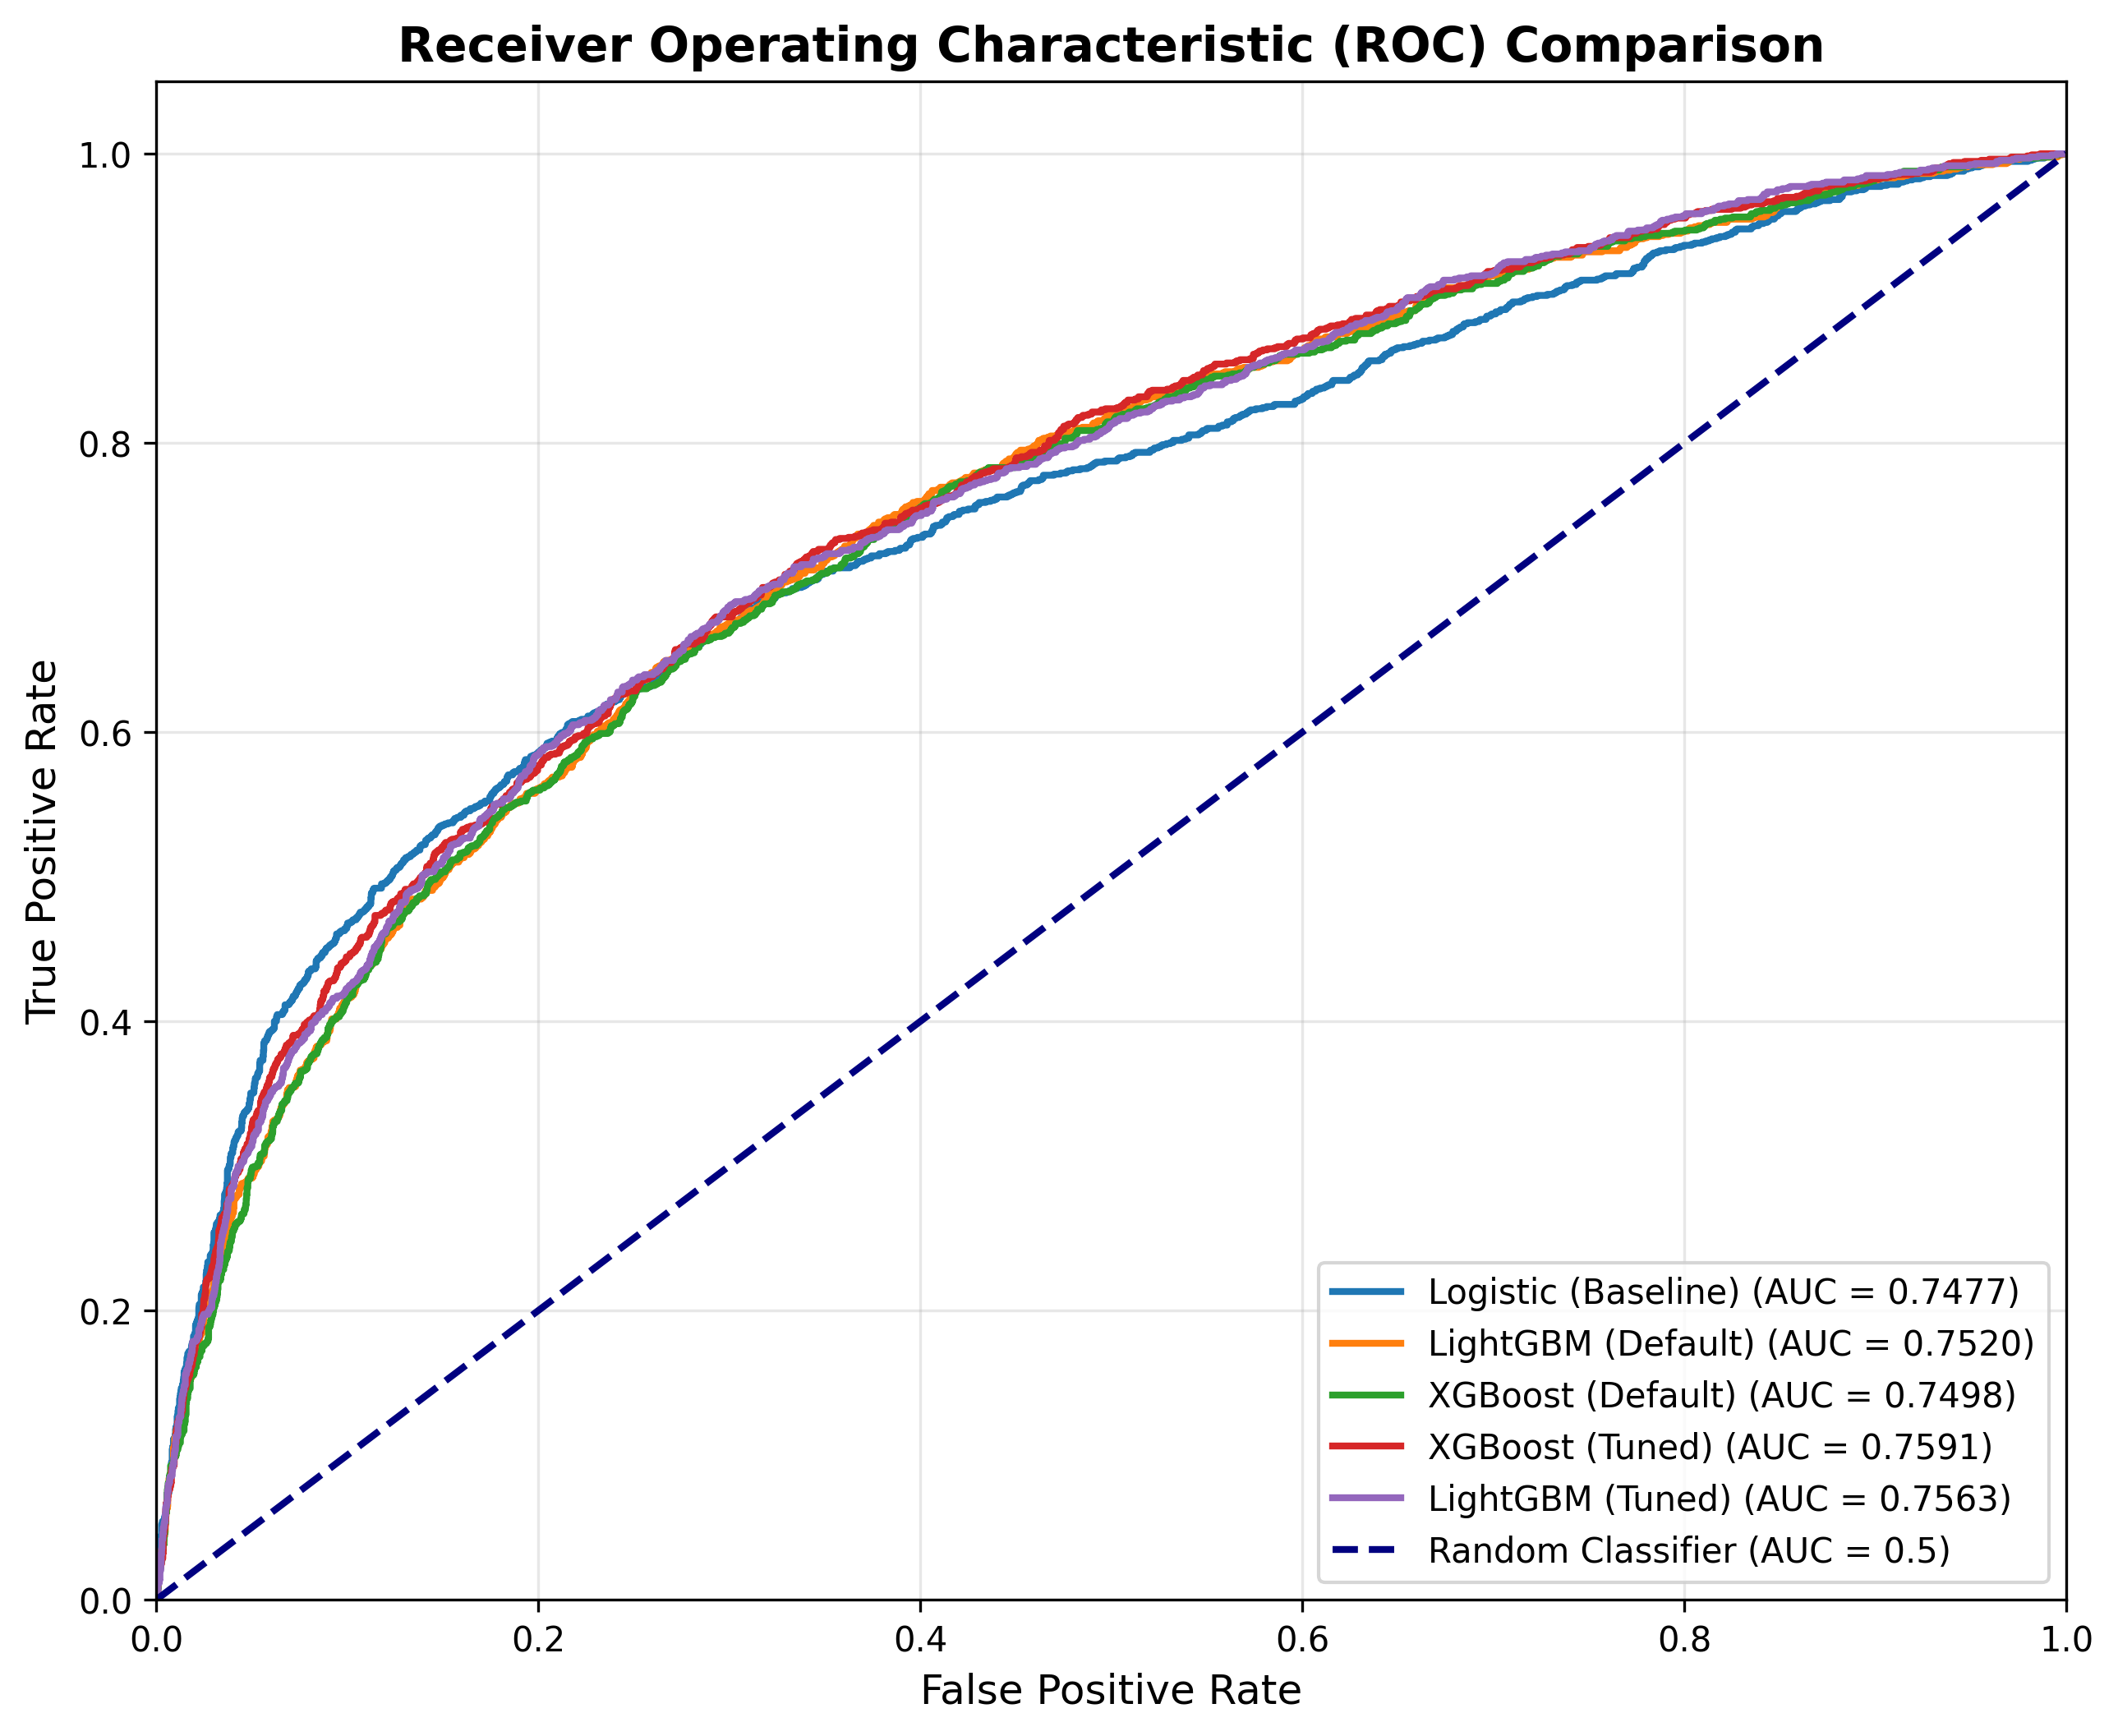
\includegraphics[width=0.85\textwidth]{../outputs/compares/final_roc_comparison.png}
    \caption{Đường cong ROC cho thấy XGBoost (Tuned) chiếm vị trí ưu thế nhất}
    \label{fig:roc_curve_all}
\end{figure}


\section{Phân tích Độ Quan Trọng của Đặc Trưng (Feature Importance)}
Việc hiểu được "tại sao" mô hình đưa ra quyết định là yếu tố then chốt để ngân hàng tin tưởng vào hệ thống AI.

\begin{figure}[H]
    \centering
    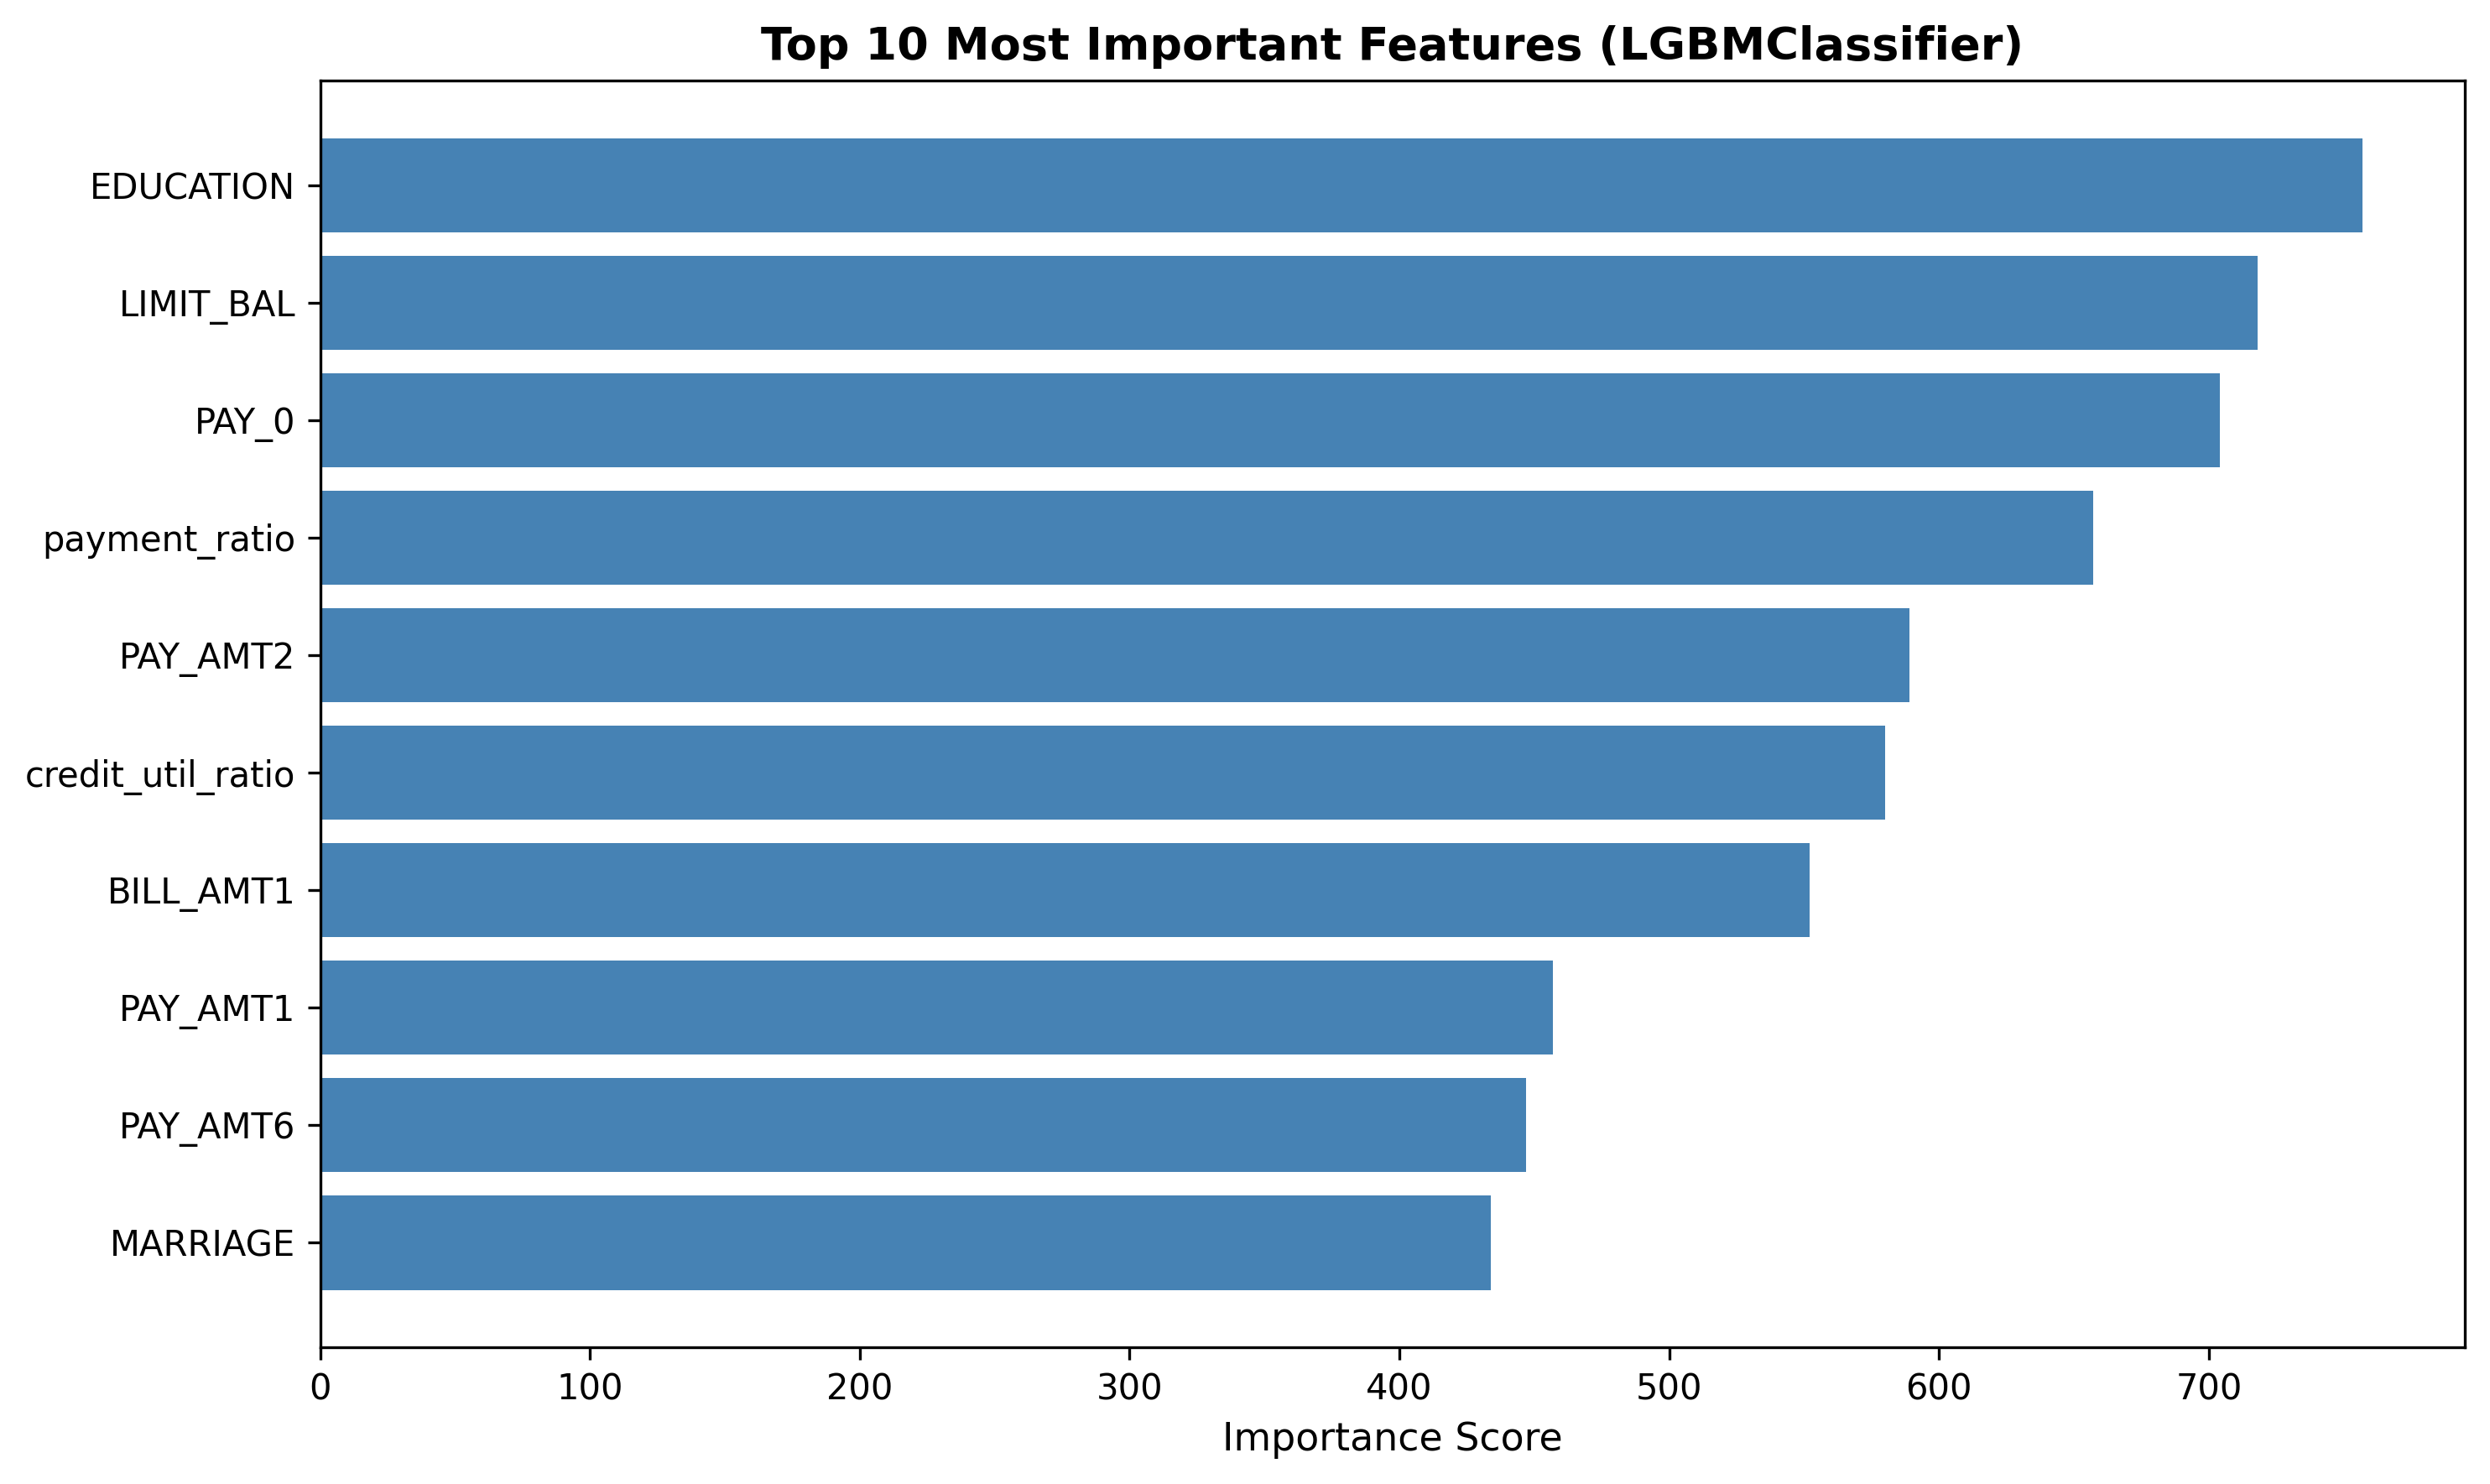
\includegraphics[width=0.95\textwidth]{../outputs/compares/feature_importance_best.png}
    \caption{Top 10 đặc trưng quan trọng nhất theo thuật toán Gains của XGBoost}
    \label{fig:feature_importance_chart}
\end{figure}

\textbf{Business Interpretation - Góc nhìn kinh doanh:} Kết quả phân tích đặc trưng mang lại những thông tin quý giá cho bộ phận quản trị rủi ro:
\begin{itemize}
    \item \textbf{Yếu tố dự báo mạnh nhất - late\_payment\_count:} Đặc trưng này chiếm vị trí áp đảo. Điều này phản ánh thực tế rằng khách hàng có thói quen trả trễ (dù chỉ vài ngày) có xu hướng lặp lại hành vi này và có nguy cơ cao chuyển thành nợ xấu thực sự. Đây là "cờ đỏ" quan trọng nhất cần theo dõi.
    \item \textbf{Lịch sử thanh toán gần nhất (PAY\_0, PAY\_2):} Trạng thái thanh toán của tháng hiện tại và tháng trước đó có trọng số cao hơn các tháng xa hơn. Điều này tuân theo nguyên tắc "Recency" trong phân tích tài chính: hành vi gần nhất phản ánh rõ nhất khả năng thanh toán hiện tại.
    \item \textbf{Sự bổ trợ của thông tin nhân khẩu học:} Mặc dù các biến hành vi chiếm ưu thế, nhưng các yếu tố như Trình độ học vấn (EDUCATION) và Tình trạng hôn nhân (MARRIAGE) vẫn đóng vai trò là các biến điều tiết, giúp mô hình phân lớp khách hàng ở mức độ chi tiết hơn.
\end{itemize}


\section{Ma trận nhầm lẫn (Confusion Matrix)}
\begin{figure}[H]
    \centering
    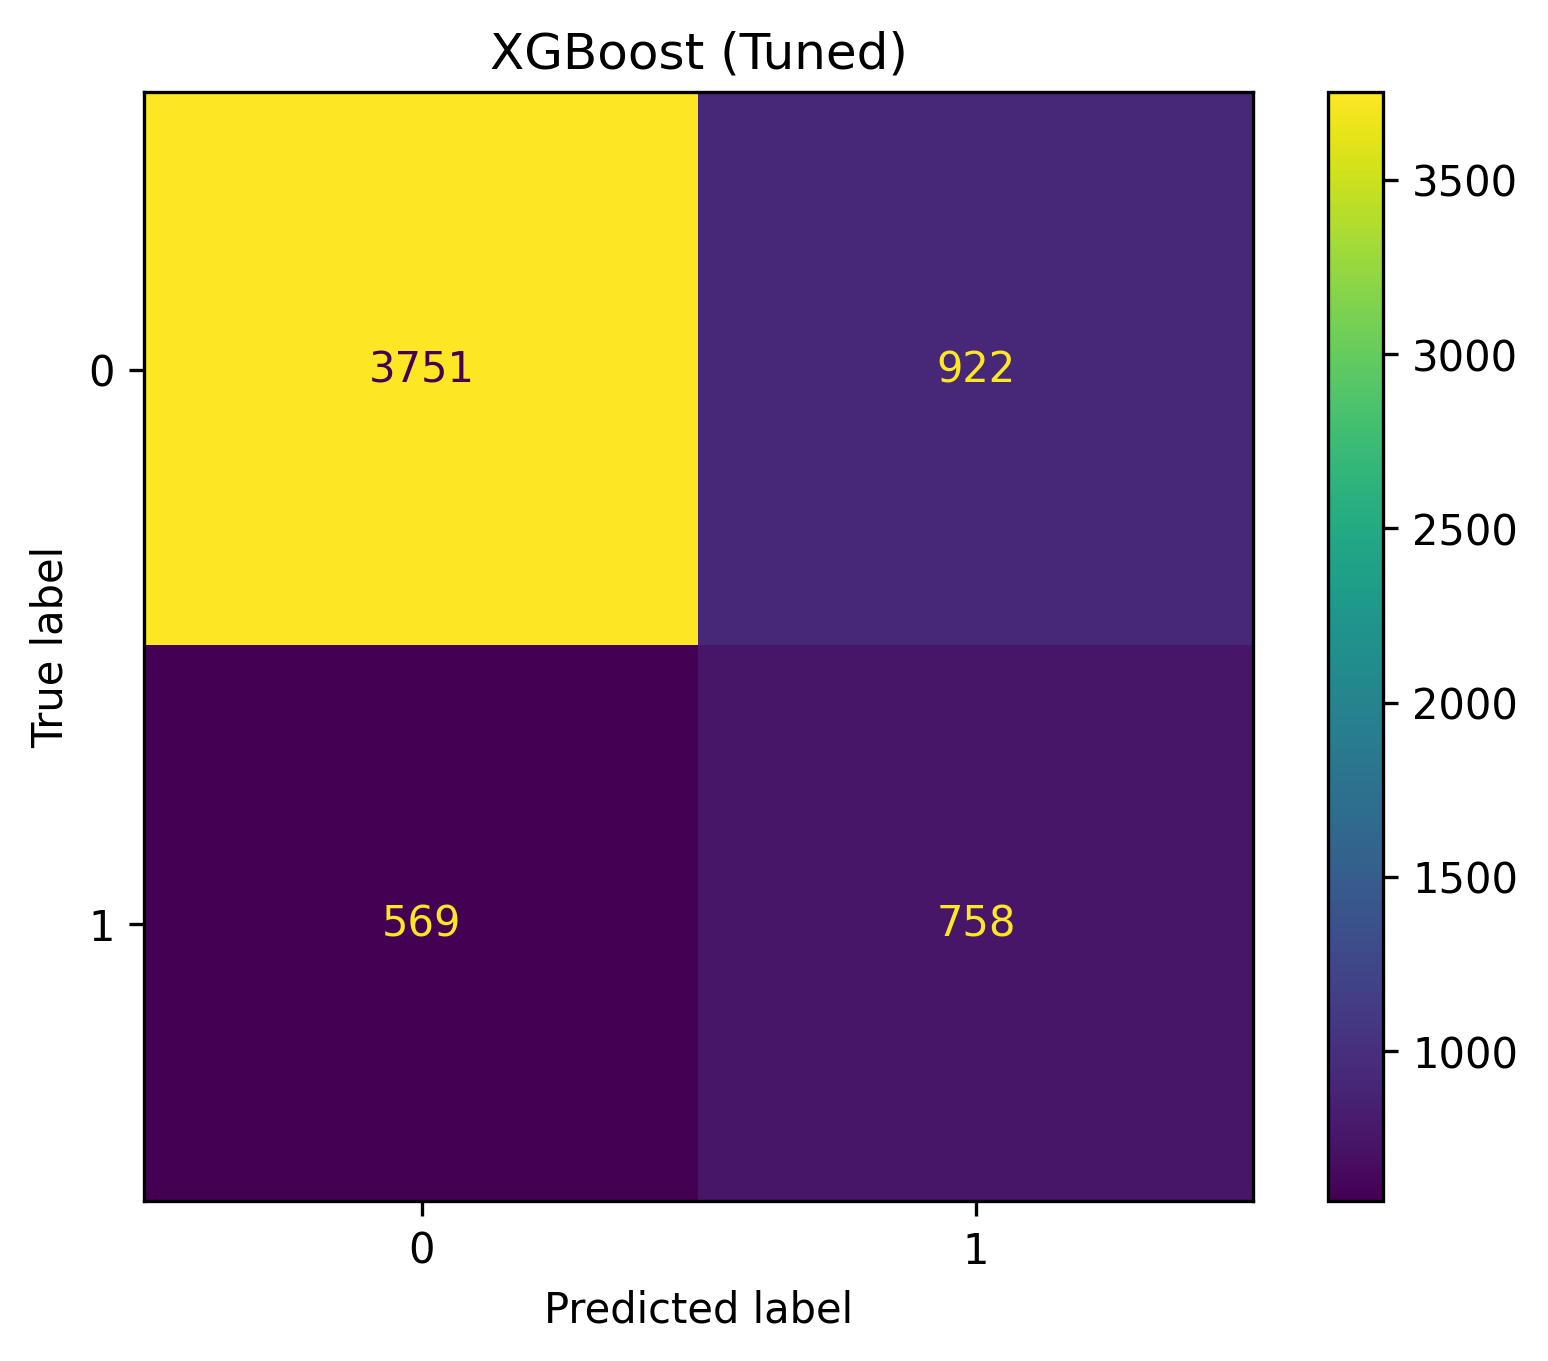
\includegraphics[width=0.48\textwidth]{../outputs/compares/confusion_xgb_tuned.png}
    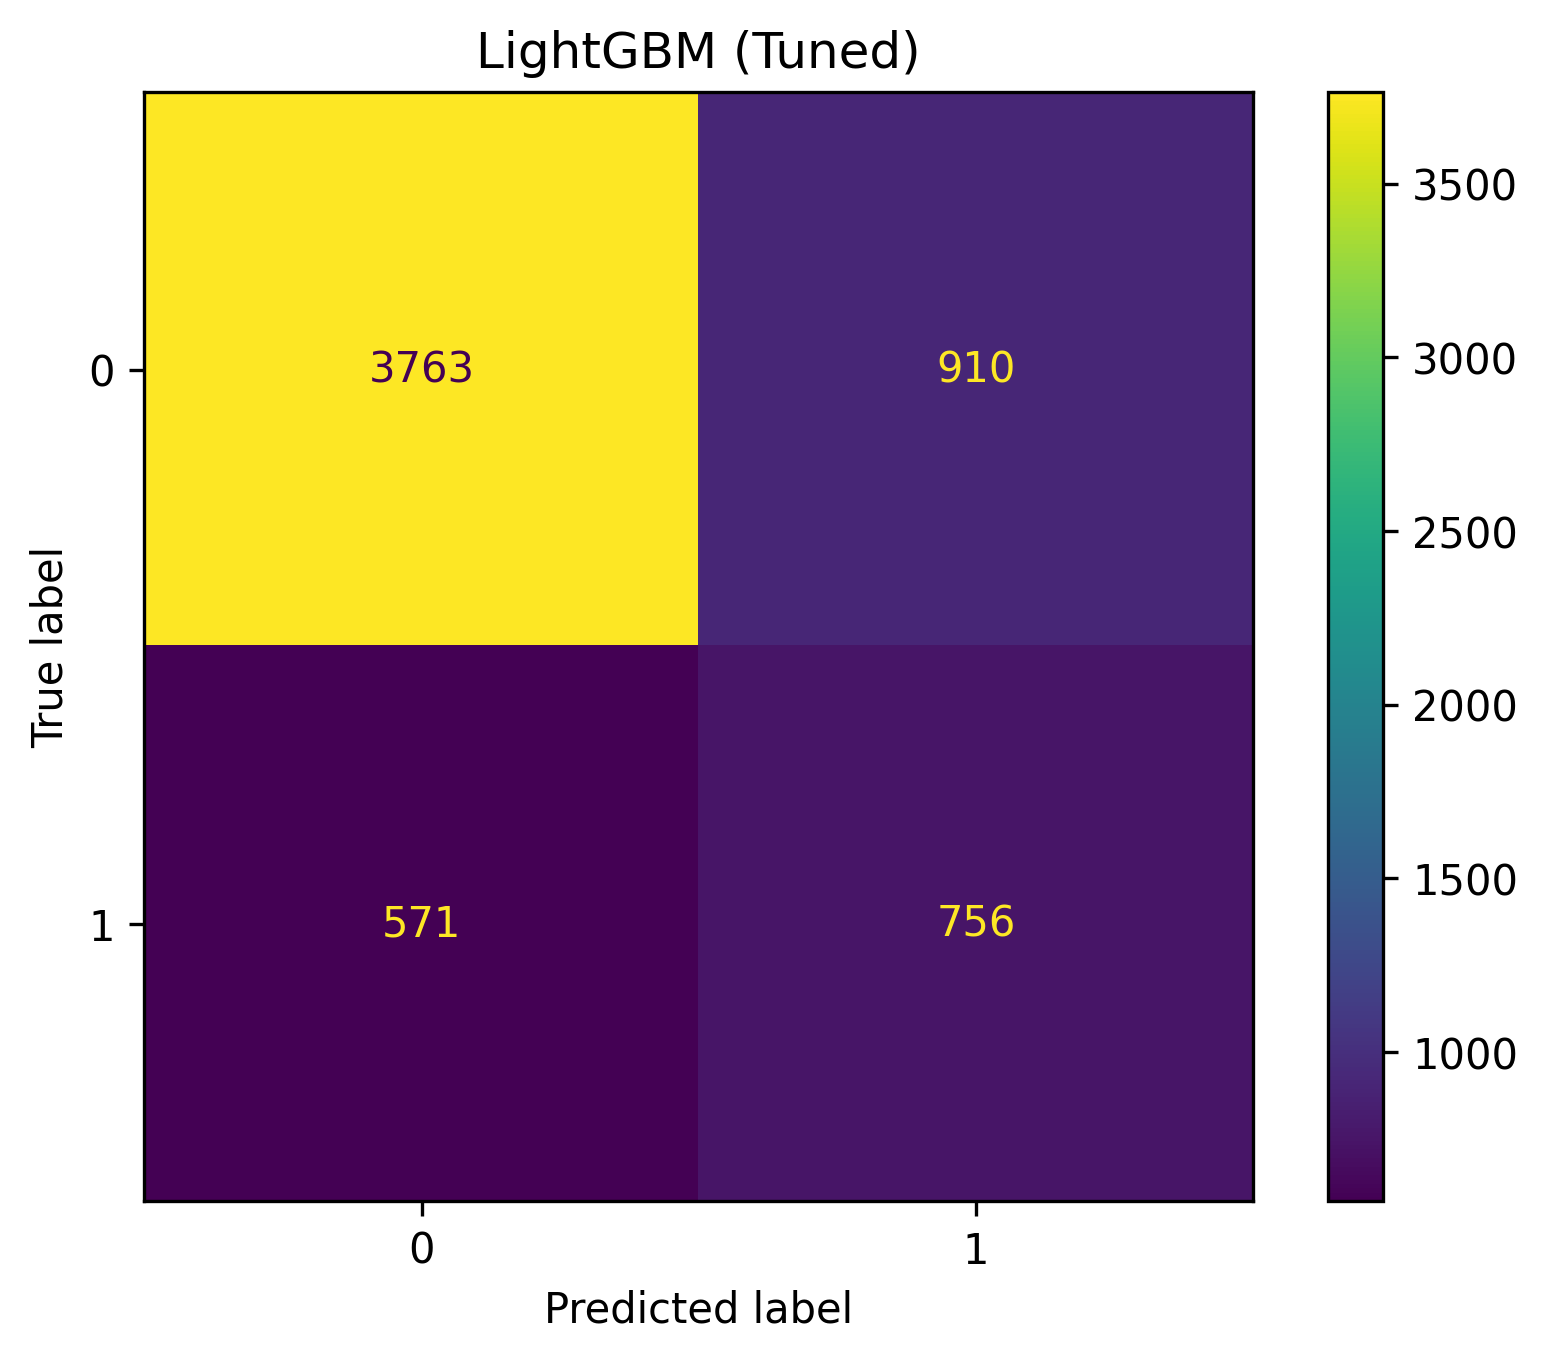
\includegraphics[width=0.48\textwidth]{../outputs/compares/confusion_lgb_tuned.png}
    \caption{Ma trận nhầm lẫn XGBoost (trái), LightGBM (phải)}
    \label{fig:confusion}
\end{figure}

\textbf{Nhận xét:} XGBoost Tuned phát hiện nhiều khách hàng nợ xấu hơn (Recall cao), phù hợp mục tiêu kiểm soát rủi ro. LightGBM Tuned cân bằng hơn giữa Recall và Precision. Cả hai đều có tỷ lệ dự báo đúng cao với nhóm khách hàng không nợ xấu. \\
\textbf{Kết luận:} Dựa trên các phân tích trên, XGBoost (Tuned) được đề xuất là mô hình chính để triển khai trong hệ thống chấm điểm tín dụng của ngân hàng, với khả năng phát hiện rủi ro vượt trội và sự giải thích rõ ràng về các yếu tố ảnh hưởng đến quyết định cho vay.
